\section{Failure Modes of Latent Space optimisation}
\label{sec:lso:limitations}
To understand the shortcomings of \gls{lmo},
it is necessary to first examine in detail the role of the generative model, which is usually a \gls{dgm}.
State-of-the-art \glspl{dgm} such as \glspl{vae} and \glspl{gan}
are trained with a prior $p(\z)$ over the latent space $\Z$.
This means that although the resulting function $g:\Z\mapsto\X$ is defined over the entire latent space $\Z$,
it is effectively only trained on points in regions of $\Z$ with high probability under $p$.
Importantly, even if $\Z$ is an unbounded space with infinite volume such as $\mathbb{R}^n$,
because $p$ has finite volume, there must exist a \emph{finite} subset $\Z'\subset\Z$ that contains virtually all the probability mass of $p$.
We call $\Z'$ the \emph{feasible region} of $\Z$.
Although in principle optimisation can be performed over all of $\Z$,
it has been widely observed that optimising outside of the feasible region tends to give poor results,
yielding samples that are low-quality, or even invalid (e.g.\@ invalid molecular strings, non-grammatical sentences);
therefore all \gls{lmo} methods known to us employ some sort of measure to restrict the optimisation to near or within the feasible region
\citep{gomez2018,kusner_grammar_2017,nguyen_synthesizing_2016,griffiths_constrained_2020,white_sampling_2016,mahmood_cold_2019,daxberger2019bayesian}.
This means that \gls{lmo} should be treated as a \emph{bounded} optimisation problem,
whose feasible region is determined by $p$.

Informally, the training objective of $g$ encourages points sampled from within the feasible region to match the data distribution that $g$
was trained on, effectively ``filling'' the feasible region with points similar to the dataset,
such that a point's relative volume is roughly proportional to its frequency in the training data.
For many optimisation problems, most of the training data for the \gls{dgm} is low-scoring
(i.e.\@ highly suboptimal objective function values),
thereby causing most of the feasible region to contain low-scoring points.
Not only does this make the optimisation problem more difficult to solve (like finding the proverbial ``needle in a haystack''),
but actually leaves insufficient space in the feasible region for a large number of novel, high-scoring points that lie outside the training distribution to be modelled by the \gls{dgm}.
Therefore, even a perfect optimisation algorithm with unlimited evaluations of the objective function
might be unable to find a novel point
that is substantially better than the best point in the original dataset,
simply because such a point may not exist in the feasible region.

\begin{figure}
    \centering
    \begin{subfigure}[c]{0.245\textwidth}
        \centering
        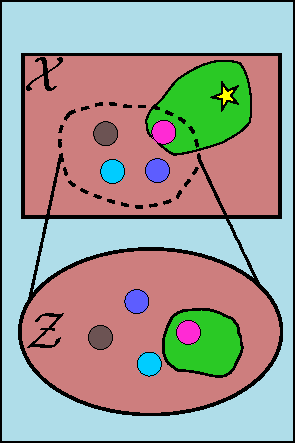
\includegraphics[width=0.9\textwidth]{schematic/base-v3.pdf}
        \vspace{-5mm}
        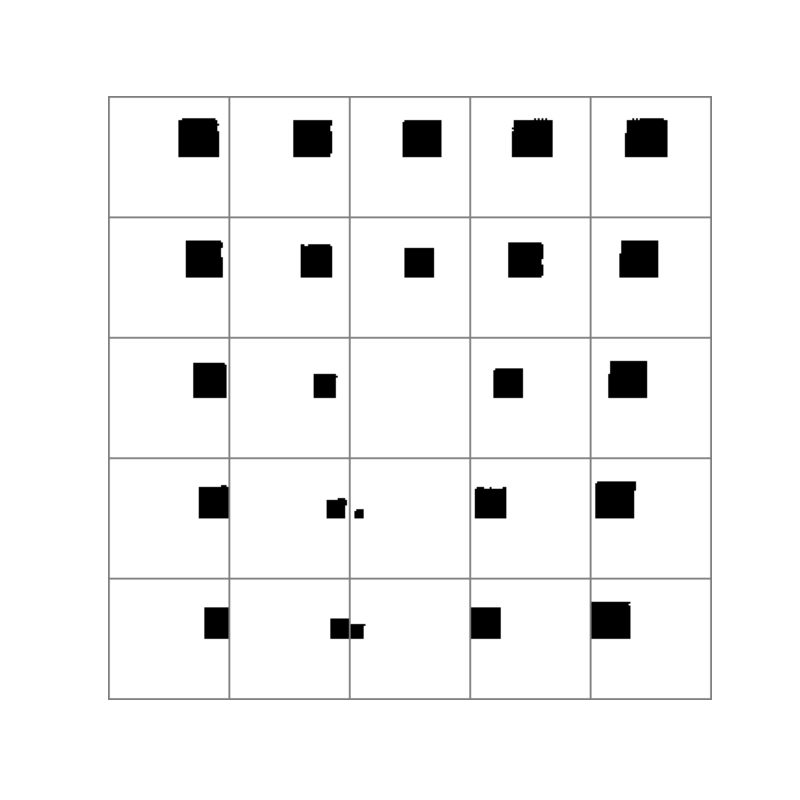
\includegraphics[width=0.95\textwidth]{schematic/shapes-manifold-plain.png}
        \subcaption{Starting Point}
        \label{subfig:lso-schematic-a}
    \end{subfigure}
    \begin{subfigure}[c]{0.245\textwidth}
        \centering
        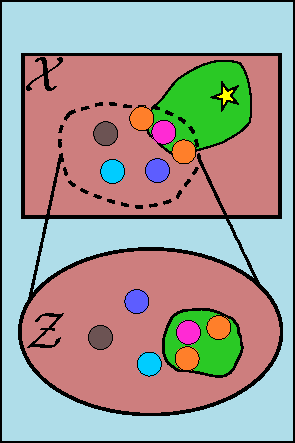
\includegraphics[width=0.9\textwidth]{schematic/normal-lso-res.pdf}
        \vspace{-5mm}
        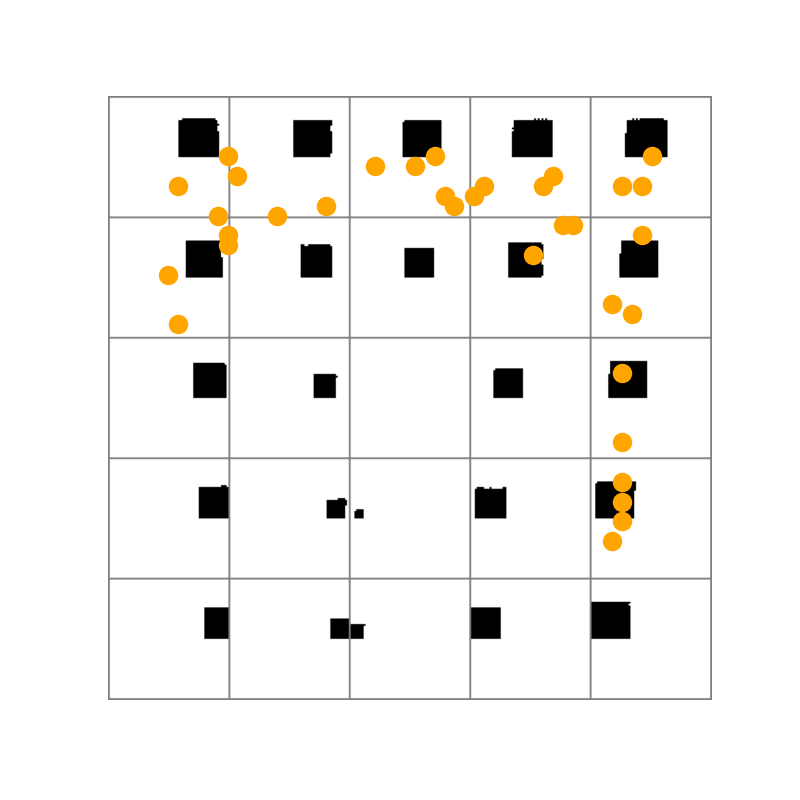
\includegraphics[width=0.95\textwidth]{schematic/shapes-manifold-plain-data.png}
        \subcaption{Standard \gls{lmo}}
        \label{subfig:lso-schematic-b}
    \end{subfigure}
    \begin{subfigure}[c]{0.49\textwidth}
        \centering
        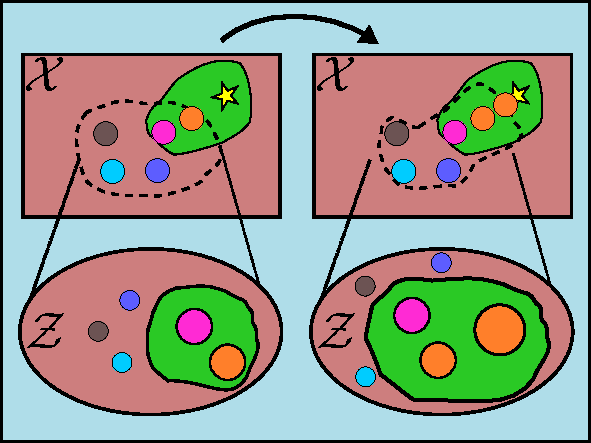
\includegraphics[width=0.9\textwidth]{schematic/wr-res.pdf}
        \vspace{-5mm}
        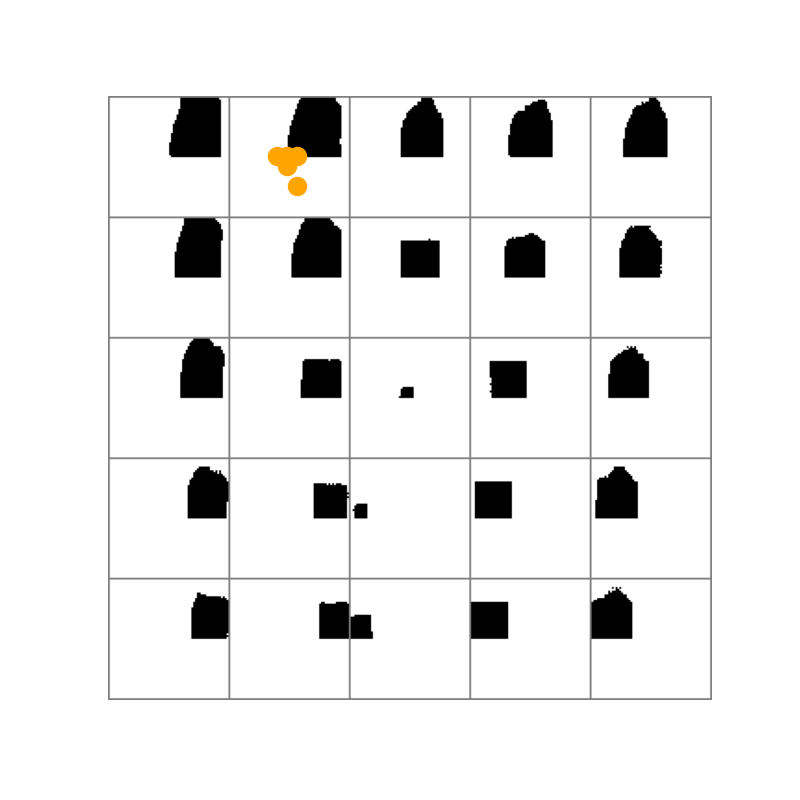
\includegraphics[width=0.475\textwidth]{schematic/shapes-manifold-wr-1.png}
        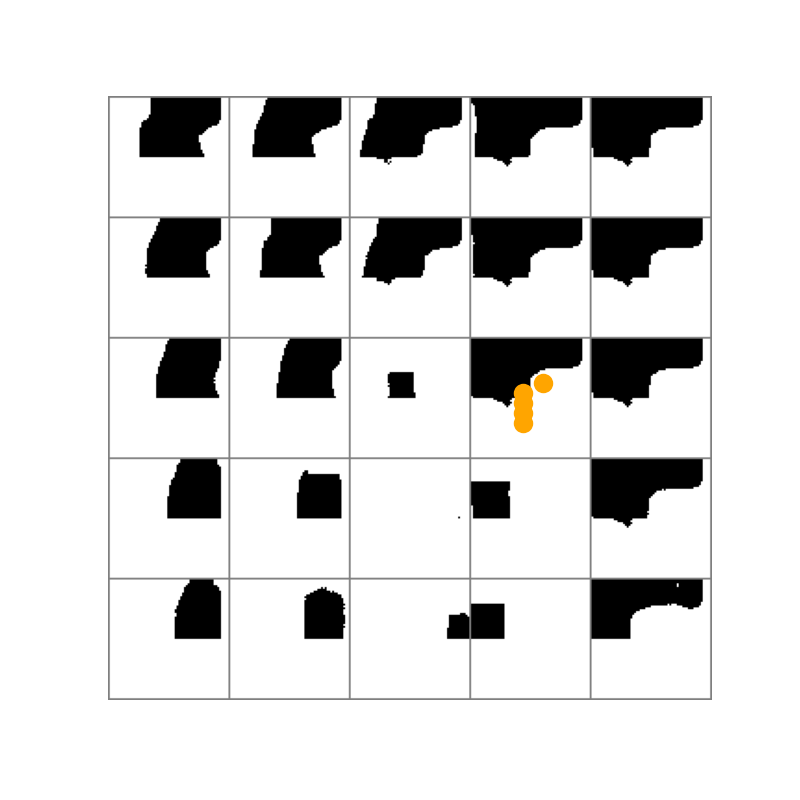
\includegraphics[width=0.475\textwidth]{schematic/shapes-manifold-wr-2.png}
        \subcaption{\Gls{lmo} with Weighted Retraining}
        \label{subfig:lso-schematic-c}
    \end{subfigure}
    \caption[Cartoon schematic of \gls{lmo}.]{
    Schematic illustrating \gls{lmo} with and without weighted retraining.
    The cartoon illustrates the input/latent space  of the generative model (\textbf{top}).
    The latent manifold from \cref{subsec:expt-wr}'s 2D shape area maximisation task is shown
    for comparison (\textbf{bottom}).
    Each image in the manifold shows the result of decoding a latent point on a uniform square grid in a 2D latent space;
    images are centred on the original grid points.
    Red/green regions correspond to points with low/high objective function values respectively.
    The yellow star is the global optimum in $\X$.
    Coloured circles are data points; their radius represents their weight.
    The dashed line surrounds the region of $\X$ modelled by $g$ (i.e.\@ $g(\Z)$, the image of $\Z$).
    \textbf{(a)} The status of the generative model $g$ at the start of optimisation.
    \textbf{(b)} The result of standard \gls{lmo} with $g$ fixed, which queries the points in orange.
    It is only able to find points close to the training data used to learn $\Z$, resulting in slow and incomplete exploration of $\mathcal{X}$.
    \textbf{(c)} The result midway (left) and at the end (right) of \gls{lmo} with our proposed approach,
    which weights data points according to their objective function value and retrains $g$ to incorporate newly queried data.
    This continually adjusts $\Z$ to focus on modelling the most promising regions of $\X$,
    speeding up the optimisation and allowing for substantial extrapolation beyond the initial training data.
    }
    \label{fig:lso-chpater-schematic}
\end{figure}

This pathological behaviour is conceptually illustrated in \cref{subfig:lso-schematic-b},
where \gls{lmo} is unable to find or even approach the global optimum that lies far from the training data.
We propose that \gls{lmo}'s performance is severely limited by two concrete problems in its setup.
The first problem is that the generative model's training objective (to learn a latent space that captures the data distribution as closely as possible),
does not necessarily match the true objective (to learn a latent space that is amenable to efficient optimisation of the objective function).
Put in terms of the cartoon in \cref{subfig:lso-schematic-b}, the feasible region that is learned, which uniformly and evenly surrounds the data points,
is not the feasible region that would be useful for optimisation,
which would model more of the green region at the expense of the red region.
This is also seen in the 2D shape area maximisation task (described in \S\ref{sec:lso:expt-tasks}).
In \cref{subfig:lso-schematic-b},
the latent manifold contains only low-area shapes that the model was trained on,
and nothing close to the all-black global optimum.
The second problem is that information on new points acquired during the iterative optimisation procedure
is not propagated to the generative model,
where it could potentially help to refine and expand the coverage of the feasible region,
uncovering new promising regions that an optimisation algorithm can exploit.
In terms of \cref{subfig:lso-schematic-b},
the new data is not used to shift the feasible region toward the green region, despite the optimisation process indicating that this is a very promising region of $\X$ for optimisation.
Luckily, we believe that neither of these two problems is inherent to \gls{lmo}, and now pose a framework that directly addresses them.
